\documentclass[a4paper]{article}
\usepackage[cm]{fullpage}
\usepackage[maxnames=6]{biblatex}
\addbibresource{../../../biblio_geosciences.bib}
\usepackage{tikz}
\usepackage{bm}
\usepackage{siunitx}
\usepackage{amsfonts}

%%%%%%%%%%%%%%%%%%%%%%%%%%%%%%%%%%%%%%%%%%%%%%%%%%%%%%%%%%%%%%%%

\title{
On the use of $Q_1\times P_0$ macro-elements for the Stokes equation with an application to 
geodynamical buoyancy-driven flows
}

\author{C. Thieulot*}


%%%%%%\keywords{Finite Elements, Stokes equations, macro-elements, buoyancy-driven flow}


\begin{document}
\maketitle

\begin{abstract}
for the first time 7 macro-elements are systematically compared in 2D on a set of benchmarks
\end{abstract}

\tableofcontents

%%%%%%%%%%%%%%%%%%%%%%%%%%%%%%%%%%%%
\section{Introduction} \label{sec1}


The Finite Element Method (FEM) is one of most popular methods in Computational Fluid Dynamics (CFD). 
When the method was first implemented 
in the early days of computers, memory limitations were severe and CFD practitioners logically 
focused on 'cheap' elements with a small memory footprint, such as the smallest velocity-pressure pair to 
solve the Stokes equations on quadrilateral: the bi/tri-linear velocity-constant pressure element, 
also denoted $Q_1 \times P_0$ (or sometimes $Q_1\times Q_0$, see \cite{grsa}). 

Unfortunately it was soon demonstrated that this element pair is not LBB-stable \cite{boni84,boni85} and this instability
manifests itself via the presence of the spurious checkerboard mode on regular meshes
which have been thoroughly analysed, see for example \cite{grsi94,chpc95,sagl81a,sagl81b}, 
despite a perfectly usable and reasonably accurate velocity field \cite{grsa,dohu03,bobf08,bobf13}.


In Gresho \& Sani \cite{grsa} it is labeled as follows: ``slightly unstable but highly usable''.
This lead some part of the community to use stable elements instead, such as the Taylor-Hood pair $Q_2\times Q_1$
(or its simplicial counterpart the $P_2\times P_1$ element \cite{thba25}), 
while the rest investigated various options to nevertheless use this element.
One can cite approaches which include a stabilizing matrix block in the lower right part of 
the otherwise empty part of the Stokes matrix\cite{kesi88,sike90,vibo92,nosi98},
the $Q_1^+\times P_0$ element of Fortin\cite{fort81}, or the $\tilde{Q}_1\times P_0$ element which adds 
a $Q_2$ bubble function to the $Q_1$ space \cite[p265]{brfo}.
Finally various stabilisations were also proposed for its 
$Q_1\times Q_1$ cousin \cite{dobo04,bodg06,busa13} but it was recently shown\cite{thba22} 
that this stabilised element is not suited to model buoyancy-driven flows, 
while retaining its usability in engineering applications.  

Arguments in favour of the $Q_1\times P_0$ element can be summarized as follows:
a) It insures mass balance at the element level \cite[p459]{grsa};
b) The pressure modes have been thoroughly analysed \cite{sagl81a,sagl81b,grsi94}.
One pressure mode is the hydrostatic mode, which is  
physical. The other one is the so-called checkerboard mode which is spurious;
c) When filtered out \cite{chpc95} the recovered pressure is usable;
d) Combined with a penalty formulation, the elimination of the pressure degrees of freedom 
yield a very compact SPD stiffness matrix \cite{zigo75,hulb79,zina82,redd82,odks82};
e) Like all other unstable elements, an irregular mesh yields a 
better numerical behaviour of the element \cite{qizh07} and pressure modes substantially subdue
(Brezzi \& Fortin p244: ``the known experimental fact that on a general
distorted mesh pressure modes disappear and the inf-sup constant is independent of h. 
This last fact is still resisting analysis.'')

Conerning the $Q_1 \times P_0$ pair, \cite{thba22} conclude:
``We believe that the $Q_1 \times P_0$ element is also not a viable
choice. As shown by several of the analytical benchmarks, the errors that result from using this element can
be orders of magnitude larger than the corresponding
errors that result from the Taylor–Hood-type elements.
This is no longer the case once we consider discontinuous viscosity profiles [...], but this element
is also unable to accurately solve the buoyancy-driven
case discussed in Sect. 5.4.''

Another option, seldom explored, is the use of so-called macro-elements composed of $Q_1\times P_0$ elements. 
Two were shown to be stable in the mid eighties\cite{leta81,sten84}, followed by three more twenty years
later\cite{qizh07} but to the author's knowledge these macro-elements were never 
implemented and compared with each other, nor put through a series of benchmarks showcasing complex flow in the 
presence of large viscosity variations/contrasts. The present article aims at 
filling this gap and drawing conlusions as to their usability also in the case of buoyancy-driven flow
since the field of computational geodynamics has long relied on the $Q_1\times P_0$ element for the 
solution of the buoyancy-driven incompressible Stokes flow in the presence of 
dominating lithostatic pressure gradient due to the Earth's gravity field.  


%%%%%%%%%%%%%%%%%%%%%%%%%%%%%%%%%%%%%%%%%%%%%%%%%%%%%%%%%%%%%
%\section{Macro-elements}\label{sec3}

Following Stenberg\cite{sten90}, we define by a macroelement $M$ ``a connected set of elements of which the 
intersection of any two is either empty, a vertex, or one edge or face in $\mathbb{R}^2$ 
and $\mathbb{R}^3$, respectively''.

In this work I focus on quadrilateral meshes and consider 8 
macro-elements, 5 from from the published literature (S, LT, QZ1, QZ2, QZ3) and 2 new ones (T1, T2) -- although 
the macro-element R fulfills the definition above it only consists of a $2\times 2$ patch of elements. 
These are shown in Figure~\ref{fig:mes}.
Note that macro-element S is often cited in the literature as example of a stable macro-element, 
e.g. \cite{chba93}+books, but rarely the LT one which in fact predates it by three years. 
Also QZ3 was mentioned in 1995 by Idehlsohn et al \cite{idsn95} but not used in calculations. 

\begin{figure}[t]
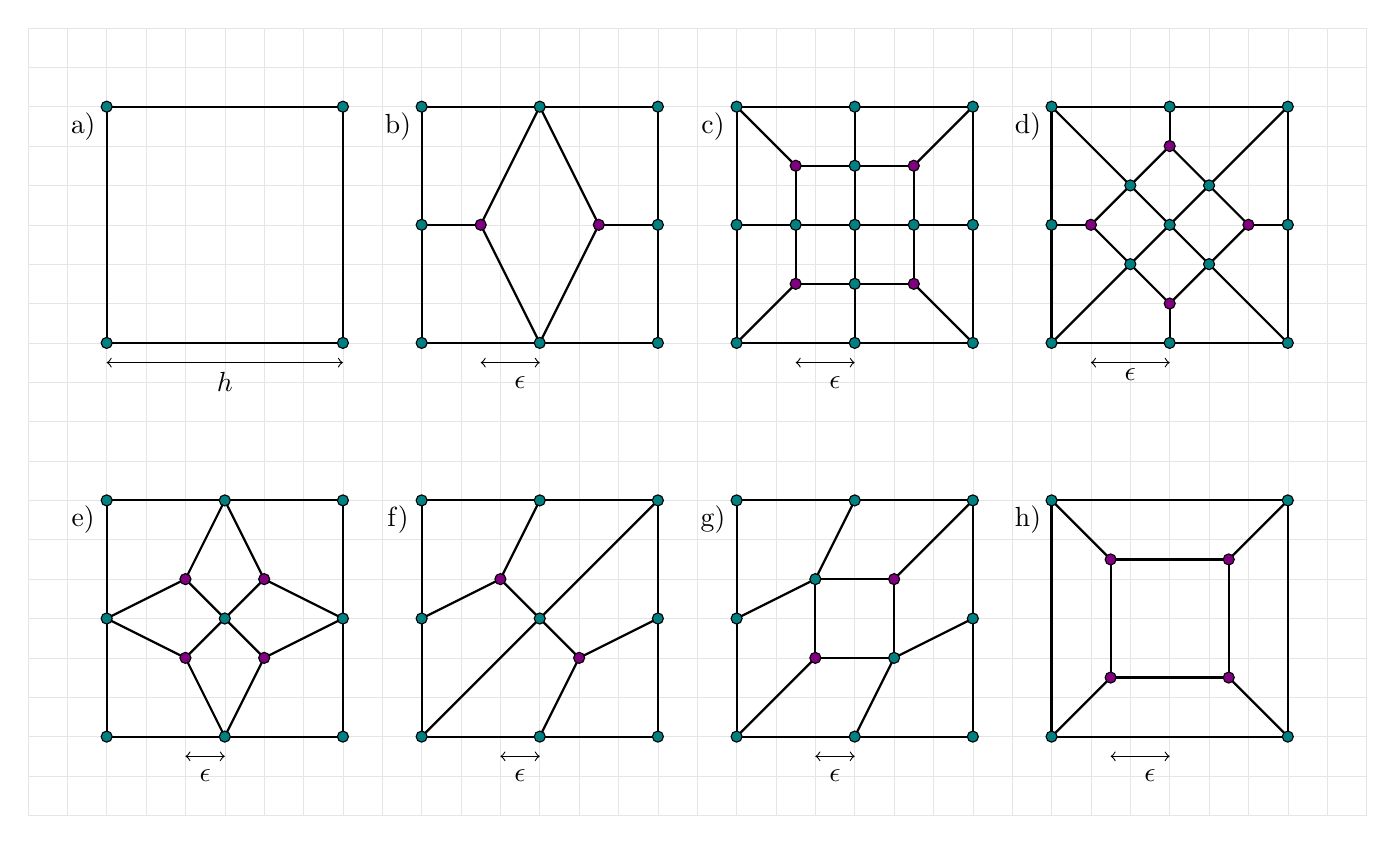
\begin{tikzpicture}
%\draw[fill=gray!23,gray!23](0,0) rectangle (5,5);
\draw[step=0.5cm,gray!20,very thin] (0,0) grid (17,10); %background grid

%%%%%%%%%%%%%%%%%%%%%%%%%%%%%%%%%%%%%%%%%%%%%%%%%%%%%%%%%%
\node[] at (0.7,3.75) {e)};
\draw[thick] (1,1) -- (4,1) -- (4,4) -- (1,4) -- cycle;  

\draw[thick] (1,2.5)--(2,3)--(2.5,4)--(3,3)--(4,2.5)--(3,2)--(2.5,1)--(2,2)--cycle;
\draw[thick] (2,2)--(3,3);
\draw[thick] (2,3)--(3,2);

\draw[black,fill=teal] (1,1)   circle (2pt);
\draw[black,fill=teal] (1,4)   circle (2pt);
\draw[black,fill=teal] (4,1)   circle (2pt);
\draw[black,fill=teal] (4,4)   circle (2pt);
\draw[black,fill=teal] (2.5,2.5)   circle (2pt);

\draw[black,fill=teal] (1,2.5)   circle (2pt);
\draw[black,fill=teal] (4,2.5)   circle (2pt);
\draw[black,fill=teal] (2.5,1)   circle (2pt);
\draw[black,fill=teal] (2.5,4)   circle (2pt);

\draw[black,fill=violet] (2,2)   circle (2pt);
\draw[black,fill=violet] (3,2)   circle (2pt);
\draw[black,fill=violet] (2,3)   circle (2pt);
\draw[black,fill=violet] (3,3)   circle (2pt);

\draw[<->] (2,0.75)--(2.5,0.75); \node[] at (2.25,0.5) {$\epsilon$};

%%%%%%%%%%%%%%%%%%%%%%%%%%%%%%%%%%%%%%%%%%%%%%%%%%%%%%%%%%%%%
\node[] at (4.7,3.75) {f)};
\draw[thick] (5,1) -- (8,1) -- (8,4) -- (5,4) -- cycle;  


\draw[thick] (6.5,1)--(7,2)--(8,2.5) ; 
\draw[thick] (5,2.5)--(6,3)--(6.5,4) ; 
\draw[thick] (6,3)--(7,2);
\draw[thick] (5,1)--(8,4);

\draw[black,fill=teal] (5,1)   circle (2pt);
\draw[black,fill=teal] (5,4)   circle (2pt);
\draw[black,fill=teal] (8,1)   circle (2pt);
\draw[black,fill=teal] (8,4)   circle (2pt);
\draw[black,fill=teal] (6.5,2.5)  circle (2pt);
\draw[black,fill=teal] (5,2.5)   circle (2pt);
\draw[black,fill=teal] (8,2.5)   circle (2pt);
\draw[black,fill=teal] (6.5,1)   circle (2pt);
\draw[black,fill=teal] (6.5,4)   circle (2pt);

\draw[black,fill=violet] (6,3)   circle (2pt);
\draw[black,fill=violet] (7,2)   circle (2pt);


\draw[<->] (6,0.75)--(6.5,0.75); \node[] at (6.25,0.5) {$\epsilon$};

%%%%%%%%%%%%%%%%%%%%%%%%%%%%%%%%%%%%%%%%%%%%%%%%%%%%%%%%%%%%%
\node[] at (8.7,3.75) {g)};
\draw[thick] (9,1) -- (12,1) -- (12,4) -- (9,4) -- cycle;  
\draw[thick] (10,2)--(11,2)--(11,3)--(10,3)--cycle; 
\draw[thick] (9,1)--(10,2);
\draw[thick] (11,3)--(12,4);
\draw[thick] (10.5,1)--(11,2)--(12,2.5);
\draw[thick] (9,2.5)--(10,3)--(10.5,4);

\draw[black,fill=teal] (9,1)   circle (2pt);
\draw[black,fill=teal] (10.5,1)   circle (2pt);
\draw[black,fill=teal] (12,1)   circle (2pt);
\draw[black,fill=teal] (9,2.5)   circle (2pt);
\draw[black,fill=teal] (12,2.5)   circle (2pt);
\draw[black,fill=teal] (9,4)   circle (2pt);
\draw[black,fill=teal] (10.5,4)   circle (2pt);
\draw[black,fill=teal] (12,4)   circle (2pt);
\draw[black,fill=teal] (10,3)   circle (2pt);
\draw[black,fill=teal] (11,2)   circle (2pt);

\draw[black,fill=violet] (10,2)   circle (2pt);
\draw[black,fill=violet] (11,3)   circle (2pt);


\draw[<->] (10,0.75)--(10.5,0.75); \node[] at (10.25,0.5) {$\epsilon$};



%%%%%%%%%%%%%%%%%%%%%%%%%%%%%%%%%%%%%%%%%%%%%%%%%%%%%%%%%%%
\node[] at (12.7,3.75) {h)};
\draw[thick] (13,1) -- (16,1) -- (16,4) -- (13,4) -- cycle;  


\draw[thick] (13.75,1.75)--(15.25,1.75)--(15.25,3.25)--(13.75,3.25)--cycle; 
\draw[thick] (13,1)--(13.75,1.75); 
\draw[thick] (16,1)--(15.25,1.75); 
\draw[thick] (13,4)--(13.75,3.25); 
\draw[thick] (16,4)--(15.25,3.25); 

\draw[black,fill=teal] (13,1)   circle (2pt);
\draw[black,fill=teal] (16,1)   circle (2pt);
\draw[black,fill=teal] (13,4)   circle (2pt);
\draw[black,fill=teal] (16,4)   circle (2pt);

\draw[black,fill=violet] (13.75,1.75)   circle (2pt);
\draw[black,fill=violet] (13.75,3.25)   circle (2pt);
\draw[black,fill=violet] (15.25,1.75)   circle (2pt);
\draw[black,fill=violet] (15.25,3.25)   circle (2pt);

\draw[<->] (13.75,0.75)--(14.5,0.75); \node[] at (14.25,0.5) {$\epsilon$};

%%%%%%%%%%%%%%%%%%%%%%%%%%%%%%%%%%%%%%%%%%%%%%%%%%%%%%%%%%%
\node[] at (0.7,8.75) {a)};
\draw[thick] (1,6) -- (4,6) -- (4,9) -- (1,9) -- cycle;  
\draw[black,fill=teal] (1,6)   circle (2pt);
\draw[black,fill=teal] (4,6)   circle (2pt);
\draw[black,fill=teal] (1,9)   circle (2pt);
\draw[black,fill=teal] (4,9)   circle (2pt);

\draw[<->] (1,5.75)--(4,5.75);
\node[] at (2.5,5.5) {$h$};

%%%%%%%%%%%%%%%%%%%%%%%%%%%%%%%%%%%%%%%%%%%%%%%%%%%%%%%%%%%
\node[] at (4.7,8.75) {b)};
\draw[thick] (5,6) -- (8,6) -- (8,9) -- (5,9) -- cycle;  
\draw[thick] (6.5,6)--(7.25,7.5)--(6.5,9)--(5.75,7.5) -- cycle;  
\draw[thick] (5,7.5) -- (5.75,7.5);  
\draw[thick] (7.25,7.5) -- (8,7.5);  
\draw[black,fill=teal] (5,6) circle (2pt);
\draw[black,fill=teal] (6.5,6) circle (2pt);
\draw[black,fill=teal] (8,6) circle (2pt);
\draw[black,fill=teal] (5,7.5) circle (2pt);
\draw[black,fill=violet] (5.75,7.5) circle (2pt);
\draw[black,fill=violet] (7.25,7.5) circle (2pt);
\draw[black,fill=teal] (8,7.5) circle (2pt);
\draw[black,fill=teal] (5,9) circle (2pt);
\draw[black,fill=teal] (6.5,9) circle (2pt);
\draw[black,fill=teal] (8,9) circle (2pt);

\draw[<->] (5.75,5.75)--(6.5,5.75); \node[] at (6.25,5.5) {$\epsilon$};


%%%%%%%%%%%%%%%%%%%%%%%%%%%%%%%%%%%%%%%%%%%%%%%%%%%%%%%%%%%%%
\node[] at (8.7,8.75) {c)};
\draw[thick] (9,6) -- (12,6) -- (12,9) -- (9,9) -- cycle;  
\draw[thick] (9.75,6.75)--(11.25,6.75)--(11.25,8.25)--(9.75,8.25) -- cycle;  

\draw[thick] (9,6) -- (9.75,6.75);  
\draw[thick] (11.25,8.25) -- (12,9);  
\draw[thick] (9,9) -- (9.75,8.25);  
\draw[thick] (11.25,6.75) -- (12,6);  
\draw[thick] (9,7.5) -- (12,7.5);  
\draw[thick] (10.5,6) -- (10.5,9);  

\draw[black,fill=teal] (9,6)  circle (2pt);
\draw[black,fill=teal] (10.5,6)  circle (2pt);
\draw[black,fill=teal] (12,6)   circle (2pt);
\draw[black,fill=teal] (9,7.5)  circle (2pt);
\draw[black,fill=teal] (10.5,7.5)  circle (2pt);
\draw[black,fill=teal] (12,7.5)   circle (2pt);
\draw[black,fill=teal] (9,9)  circle (2pt);
\draw[black,fill=teal] (10.5,9)  circle (2pt);
\draw[black,fill=teal] (12,9)   circle (2pt);

\draw[black,fill=teal] (10.5,8.25)   circle (2pt);
\draw[black,fill=teal] (10.5,6.75)   circle (2pt);
\draw[black,fill=teal] (9.75,7.5)   circle (2pt);
\draw[black,fill=teal] (11.25,7.5)   circle (2pt);

\draw[black,fill=violet] (9.75,6.75)  circle (2pt);
\draw[black,fill=violet] (11.25,6.75)  circle (2pt);
\draw[black,fill=violet] (9.75,8.25)  circle (2pt);
\draw[black,fill=violet] (11.25,8.25)  circle (2pt);


\draw[<->] (9.75,5.75)--(10.5,5.75); \node[] at (10.25,5.5) {$\epsilon$};


%%%%%%%%%%%%%%%%%%%%%%%%%%%%%%%%%%%%%%%%%%%%%%%%%%%%%%%%%%%
\node[] at (12.7,8.75) {d)};
\draw[thick] (13,6) -- (16,6) -- (16,9) -- (13,9) -- cycle;  

\draw[thick] (13,6) -- (16,9) ;
\draw[thick] (13,9) -- (16,6) ;

\draw[thick] (13.5,7.5)--(14.5,6.5)--(15.5,7.5)--(14.5,8.5) -- cycle;
\draw[thick] (13,7.5) -- (13.5,7.5) ;
\draw[thick] (15.5,7.5) -- (16,7.5) ;
\draw[thick] (14.5,6) -- (14.5,6.5) ;
\draw[thick] (14.5,8.5) -- (14.5,9) ;

\draw[black,fill=teal] (13,6)   circle (2pt);
\draw[black,fill=teal] (14.5,6)   circle (2pt);
\draw[black,fill=teal] (16,6)   circle (2pt);
\draw[black,fill=teal] (13,7.5)   circle (2pt);
\draw[black,fill=teal] (14.5,7.5)   circle (2pt);
\draw[black,fill=teal] (16,7.5)   circle (2pt);
\draw[black,fill=teal] (13,9)   circle (2pt);
\draw[black,fill=teal] (14.5,9)   circle (2pt);
\draw[black,fill=teal] (16,9)   circle (2pt);

\draw[black,fill=teal] (14,7)   circle (2pt);
\draw[black,fill=teal] (15,7)   circle (2pt);
\draw[black,fill=teal] (14,8)   circle (2pt);
\draw[black,fill=teal] (15,8)   circle (2pt);

\draw[black,fill=violet] (14.5,6.5)   circle (2pt);
\draw[black,fill=violet] (14.5,8.5)   circle (2pt);
\draw[black,fill=violet] (13.5,7.5)   circle (2pt);
\draw[black,fill=violet] (15.5,7.5)   circle (2pt);

\draw[<->] (13.5,5.75)--(14.5,5.75); \node[] at (14,5.6) {$\epsilon$};

\end{tikzpicture}

\caption{
a) velocity and pressure nodes for a $Q_1\times P_0$ element;
b) Stenberg (S) macro-element \cite{sten84}; 
c) Le Tallec (LT) macro-element \cite{leta81,leru86}; 
d,e,f) Qin \& Zhiang (QZ1, QZ2, and QZ3) macro-elements \cite{qizh07}; 
g,h) newly proposed macro-elements T1 and T2 (this study).
Velocity nodes are represented by filled-in circles. The purple ones indicate internal nodes which belong to 3 elements.
For each macro-element a distance $\epsilon$ is indicated which controls the positioning of the internal nodes.
\label{fig:mes}}
\end{figure}

Note that the new macro-elements proposed by the author have not been proven stable. They are arrived at 
observing the other existing ones and making sure that they contain at least one node that belongs to three 
elements so as to hamper checkboard modes.

%checkerboard: US
%chequerboard: UK

Looking  at Fig~\ref{fig:mes}, we can also make the observation that some macro-elements 
have a two-fold symmetry (along the axis or the diagonals) while others have a four-fold one 
(axis and diagonals). May be more important is the fact that S, QZ3 and A are 'anisotropic', i.e., in 
the case of QZ3 for example, there is an edge joining two opposite corners but none joining the 
other two opposite corners.
In Table~\ref{tab1} I summarize the various properties which characterizes each macro-element.

\begin{table}
\centering
\begin{tabular}{cccccc}
\hline
{name} & {axes symmetry}  & {diagonals symmetry} & {\# add. nodes inside} 
& {\# elements per m-e} & {mid edge points}  \\
\hline
\hline
R   &  Yes &  Yes & 1  & 4 & No \\
S   &  Yes &   No & 2  & 5 & Yes \\
LT  &  Yes &  Yes & 9 & 12 & Yes \\
QZ1 &  Yes &  Yes & 9 & 12 & Yes \\
QZ2 &  Yes &  Yes & 5 & 8  & Yes \\
QZ3 &  No  &  Yes & 3 & 6  & Yes \\
A   &  No  &  Yes & 4 & 7  & Yes \\
B   &  Yes &  Yes & 4 & 5  & No  \\
\hline
\end{tabular}
\caption{Characteristics of all 8 macro-elements as shown in Fig.~\ref{fig:mes}.\label{tab1}}%
\end{table}

The stability of a velocity-pressure pair or a macro-element is often difficult to prove 
and various techniques have been proposed \cite{bobf13}. 
All 5 published macro-elements were shown to be LBB-stable and all showcase at least 
an internal node shared by an odd number of elements which makes a chequerboard pattern impossible. 
However, things are not that simple since macro-element T2 showcases 
4 such points and as we will see it is not stable and chequerboard patterns still occur 
albeit at the macro-element scale (I have used the macro-element technique of Stenberg 
also in Lamichhane to show that a patch of 2x2 m-e of T2 type have indeed a chequerboard mode). {\color{red} REDO?!}
Looking at a macro-element is therefore not sufficient to determine whether it is LBB-stable or not. 

Qi et al \cite{qizh07} state "[...] from the points of implementation and the approximation property, we 
would list five types of macro-elements from the best to worst as S, LT, QZ1, QZ2, QZ3." 
The authors unfortunately do not provide any numerical comparison between these 5 and their 
ranking is therefore not borne by hard evidence. Furthermore, we will find that our ranking disagrees with theirs. 
%Understand what their ranking is based on. My pragmatic approach - numerical testing!

\paragraph{A remark about the QZ1 and QZ3 macro-elements:}
Let us consider the triangular macro-element as shown in Fig.~\ref{fig:triangle}.
As mentioned in \cite{rovira1992}, 
the velocity and pressure spaces in this case are isomorphic to those
of the $P_2^+ \times P_{-1}$ element \cite{thba25}. Since this velocity-pressure pair 
element satisfies the LBB condition, the macroelement depicted in this figure
composed of $Q_1 \times P_0$ elements is also be div-stable.

\begin{figure}
\centering
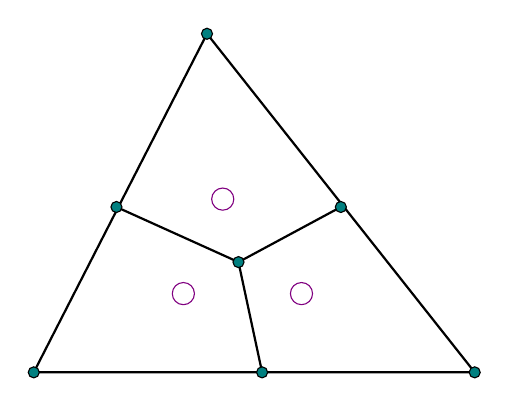
\begin{tikzpicture}
\draw[thick] (0,0) -- (5.6,0) -- (2.2,4.3)-- cycle;  
\draw[thick] (1.05,2.1) -- (2.6,1.4) -- (3.9,2.1);  
\draw[thick] (2.6,1.4) -- (2.9,0);  
\draw[black,fill=teal] (0,0) circle (2pt);
\draw[black,fill=teal] (5.6,0) circle (2pt);
\draw[black,fill=teal] (2.2,4.3) circle (2pt);
\draw[black,fill=teal] (1.05,2.1) circle (2pt);
\draw[black,fill=teal] (2.6,1.4) circle (2pt);
\draw[black,fill=teal] (3.9,2.1) circle (2pt);
\draw[black,fill=teal] (2.9,0) circle (2pt);
\draw[violet] (1.9,1) circle (4pt);
\draw[violet] (3.4,1) circle (4pt);
\draw[violet] (2.4,2.2) circle (4pt);
\end{tikzpicture}
\caption{A triangular macro-element made of 3 $Q_1\times P_0$ elements.
Green discs correspond to velocity nodes while open circle correspond to pressure dofs.}\label{fig:triangle}
\end{figure}

\vspace{.4cm}


In the end, despite the existing literature, many questions remain with regards to these macro-elements:
\begin{itemize}
\item Based on a handful of benchmarks is it possible to establish a ranking, or at the very least can we pinpoint the objectively worse one(s)?

\item Is there an optimal position for the additional internal nodes? (i.e. can we determine an optimal value of the 
$\epsilon$ parameter for each macro-element?)

\item Can these macro-elements be safely used for geodynamical 
buoyancy-driven flows in the presence of a strong hydrostatic pressure gradient?
\end{itemize}











%%%%%%%%%%%%%%%%%%%%%%%%%%%%%%%%%%%%%%%%%%%%%%%%%%%%%%%%%%%%%%%%%%%%%%%%%5
\section{Implementation}


For the purpose of this paper, we are concerned with the numerical solution of 
the incompressible and isothermal Stokes equations:
\begin{eqnarray}
-\nabla \cdot \left[ 2\eta \dot\varepsilon({\bm u}) \right] + \nabla p &=& \rho \bm g \qquad  \textrm{in $\Omega$},
\label{eq:conv_momentum}  \\  
-\nabla \cdot {\bm u} &=& 0    \qquad    \textrm{in $\Omega$},   \label{eq:conv_mass} 
\end{eqnarray}
where $\eta$ is the viscosity, $\rho$ the density, ${\bm g}$ the gravity vector, $\dot\varepsilon(\cdot)$
denotes the symmetric gradient operator defined by $\dot\varepsilon({\bm u})
=\frac 12 (\nabla {\bm u} + \nabla {\bm u}^{T})$, 
and $\Omega\subset{\mathbb R}^d, d=2\text{ or }3$ is the domain
of interest. Both the viscosity $\eta$
and the density $\rho$ will, in general, be spatially variable.

In this paper the Stokes equations are discretised using the finite element method.
The unknowns are the velocity vector ${\bm u}$ and the pressure $p$ so that 
one speaks of a Mixed Finite Element method. 
A straightforward application of the Galerkin method yields the finite-dimensional 
variational problem: 
\textit{Find ${\bm u}_h\in {\cal Q}_1,p_h\in {\cal Q}_0$
so that
\begin{eqnarray}
\label{eq:discrete-formulation}
\left(\varepsilon(\bm v_h), 2\eta \varepsilon(\bm u_h)\right)  - ( \nabla \cdot \bm v_h, p_h) &=&   ({\bm v}_h,\rho \bm g),\\
-(q_h,\nabla \cdot \bm u_h) &=& 0,
\end{eqnarray}
for all test functions ${\bm v}_h\in {\cal Q}_1, q_h\in {\cal Q}_0$.}
This procedure is rather standard and well documented in many 
textbooks \cite{grsa,dohu03,bobf13} and the reader is referred to these sources 
for more detail.

All (macro-)elements have been implemented in a dedicated Python code (see Supplementary material). 
An isoparametric mapping is used. 
The fully assembled Stokes matrix is passed to a Python solver (WHICH exactly). 
Better solving strategies have of course 
been designed to solve the resulting saddle point \cite{begl05} but are not 
implemented since optimal performance is not of interest here.
The pressure nullspace due to the Dirichlet boundary conditions on all sides is removed 
after the linear system is solved, by imposing $\int_\Omega p dV= 0$.

The projection of the discontinuous pressure $p$ onto the velocity nodes is denoted by $q$. 
Techniques how to do so (and thereby filter out the checkerboard modes) have been presented in 
\cite{chpc95,legs79}.
For simplicity I have adopted the simple procedure explained in \cite{REF}: each 
elemental pressure is added to the nodes making this element and later averaged. 

When an analytical solution exists convergence rates are computed and 
we expect for smooth viscosity fields and/or boundary conditions that the convergence rates 
are optimal, i.e., that the errors satisfy the relationships
\begin{eqnarray}
\| {\bm u} - {\bm u}_h \|_{L_2} &=&  {\cal O}(h^{2}),     \\  
\| p - p_h \|_{L_2}   &=& {\cal O}(h^{1}),
  \label{eq:error-rates}
\end{eqnarray}
where $h$ is the average diameter over all cells in the mesh.
I will also measure and report on the convergence rate index for the nodal pressure $q$.

Looking at Fig.~\ref{fig:mes} we see that the elements inside the macro-elements 
have various sizes and shapes so 
the default version of each macro-element is the one for which all internal elements have the same area
(when possible -- see appendix), and I then define the average element size
$\langle h \rangle$ as the square root of the average elemental area.


%%%%%%%%%%%%%%%%%%%%%%%%%%%%%%%%%%%%%%%%%%%%%%%%%%%%%%%%%%%%%%%%%%
\section{The Donea \& Huerta manufactured solution as test case}

To test the implementation I first consider the manufactured solution 
proposed in Chapter 6 of \cite{dohu03} and also used in \cite{thba22,thba25}.
 
The domain is a unit square. The viscosity is set to $\eta=1$.
The velocity and pressure fields are given by
\begin{eqnarray}
u_x(x,y) &=& x^2(1- x)^2 (2y - 6y^2 + 4y^3)  \\
u_y(x,y) &=& -y^2 (1 - y)^2 (2x - 6x^2 + 4x^3) \\
p(x,y) &=& x(1 -x)- 1/6. 
\end{eqnarray}
The buoyancy force is obtained by inserting these expressions in Eq.~\ref{eq:conv_momentum}.
Boundary conditions are no-slip on all sides of the domain.

The velocity and pressure fields obtained with a subset of the macro-elements 
are shown in Fig.~\ref{fig:dh1}


\begin{figure}[t]
{\color{red} insert vel, p field, for R,S,T2}
\caption{ \label{fig:dh1}}
\end{figure}

\begin{figure}
\centering
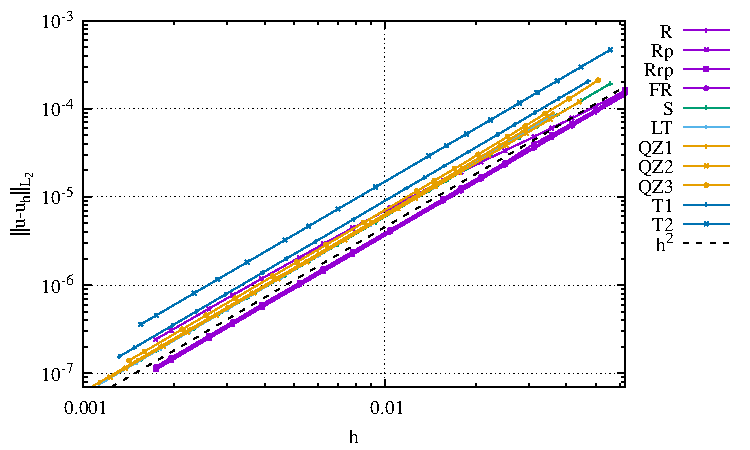
\includegraphics[width=8cm]{../results/errors_u_exp1}
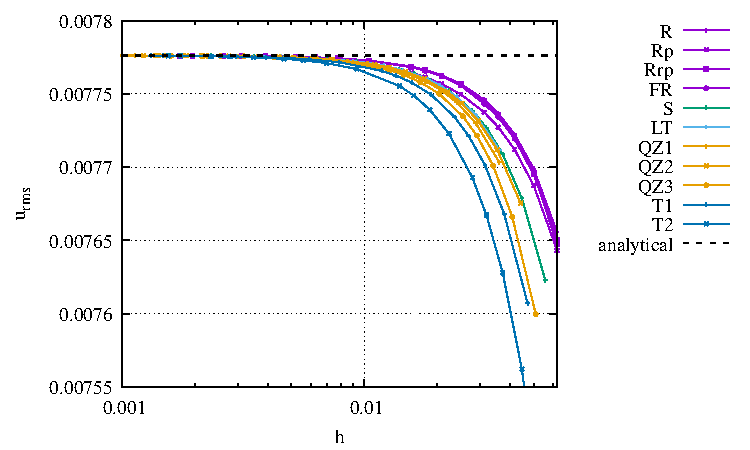
\includegraphics[width=8cm]{../results/vrms_exp1} \\
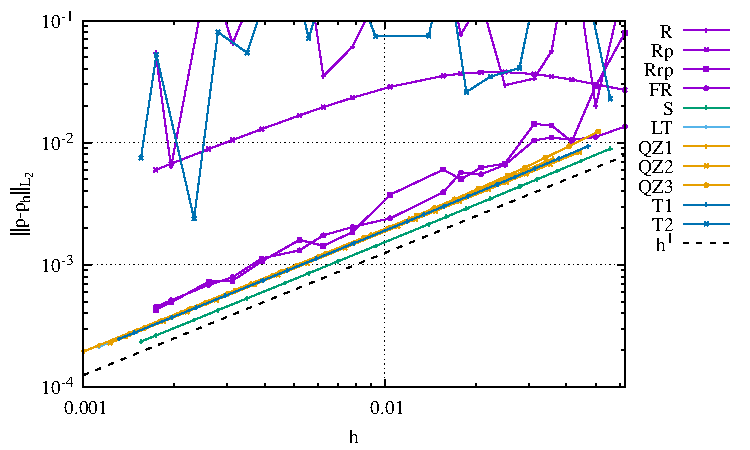
\includegraphics[width=8cm]{../results/errors_p_exp1}
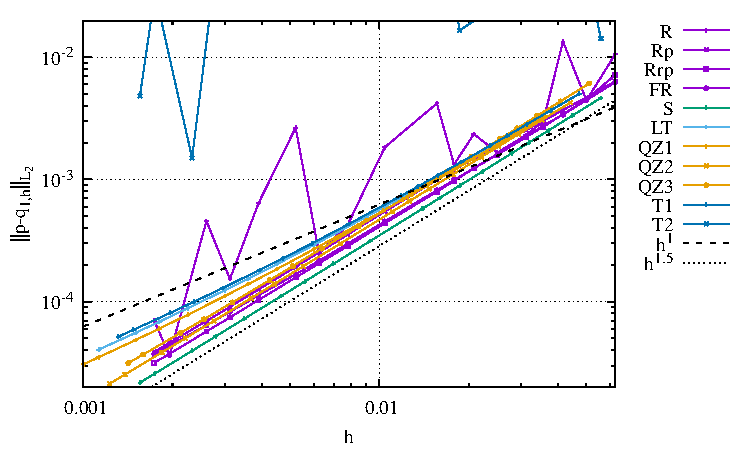
\includegraphics[width=8cm]{../results/errors_q1_exp1}
\caption{Donea and Huerta benchmark: velocity error, 
root mean square velocity, elemental pressure error and nodal pressure error
as a function of the the average mesh size $h$.} 
\label{fig:resdh}
\end{figure}




In Fig.~\ref{fig:resdh} the velocity and pressure errors are shown as a function of the 
average mesh size $\langle h \rangle$ for all 8 macro-elements.

\begin{itemize}

%comment on velocity
\item We recover optimal rates for velocity ${\bm u}$ (quadratic convergence) for all macro-elements.
The 'R' macro-element is the most accurate, followed by S, LT, QZ1, QZ2, QZ3 which are very close, 
while the T1 and T2 macro-elements are the least accurate ones. 
%comment on vrms
\item All macro-elements converge to the correct root mean square velocity $u_{rms}$ and 
their accuracy follows the previously made observations on their respective velocity errors.

%comment on elemental pressure p
\item As expected the 'R' macro-element yields a pressure field showcasing a checkerboard so that 
the corresponding pressure error does not decrease with increasing $<h>$. 
\item The same observation can be made for macro-element 'T2'. 
\item All other macro-elements pressure errors converge linearly and the 'S' macro-element is
the most accurate of them all.
\item The amplitude of checkerboard modes is difficult to predict (it is a function 
of boundary conditions, mesh topology, even or odd numbers of elements per direction, flow features, ...) \cite{XXX} 

%comment on nodal pressure q
\item Because the 'R' and 'T2' macro-elements yield a checkerboard pressure field, we need not
assessing their nodal projection and these have then been removed from Fig.~\ref{fig:resdh}c.
\item A handfull of macro-elements (S, QZ2, QZ3) have their nodal pressure $q$ converge like ${\cal O}(h^{1.5})$
while the others (LT, QZ1, T1) ultimately see their nodal pressure converge linearly.
\item Again, 'S' is the most accurate of them all.

\end{itemize}


The newly-proposed macro-element T2 is not stable as the checkboard pattern is clearly visible in Fig.~\ref{fig:check}. 
Also, this macro-element also always yields the worse velocity error. It is therefore abandonned in what follows. 
As a conclusion, S is the clear best macro-element, followed by QZ2 and QZ3 macro-elements.

{\color{red} TODO: I need to re-do all this with different mms and see whether this holds!!}


%%%%%%%%%%%%%%%%%%%%%%%%%%%%%%%%%%%%%%%%%%%%%%%%%%%%%%%%%%
\section{Non-isoviscous manufactured solutions}





\begin{figure}
\centering
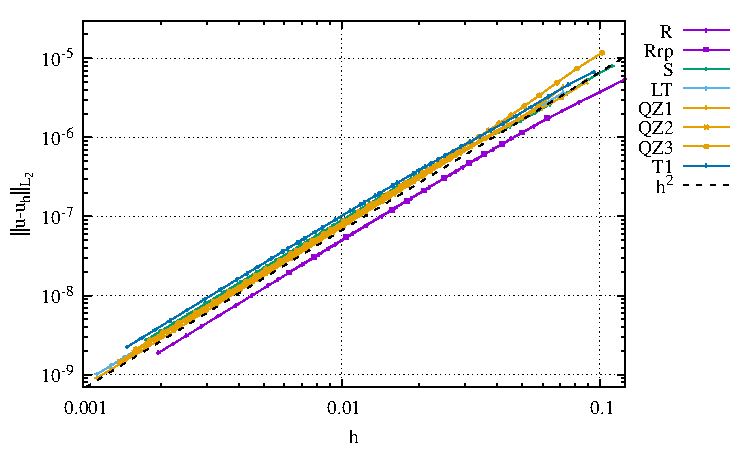
\includegraphics[width=8cm]{../results/errors_u_exp5}
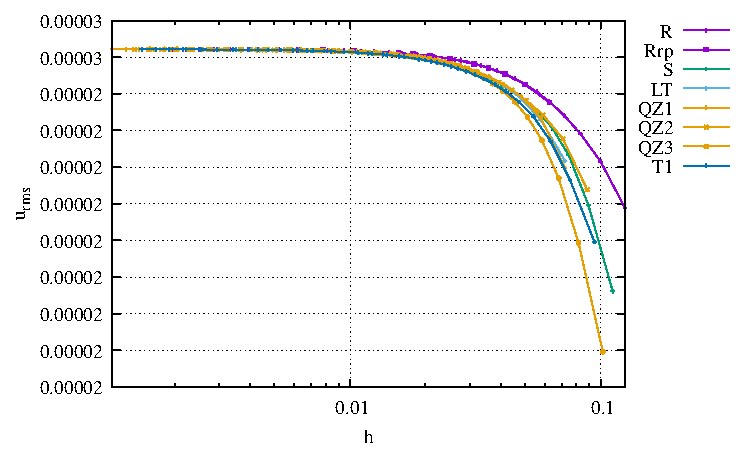
\includegraphics[width=8cm]{../results/vrms_exp5} \\
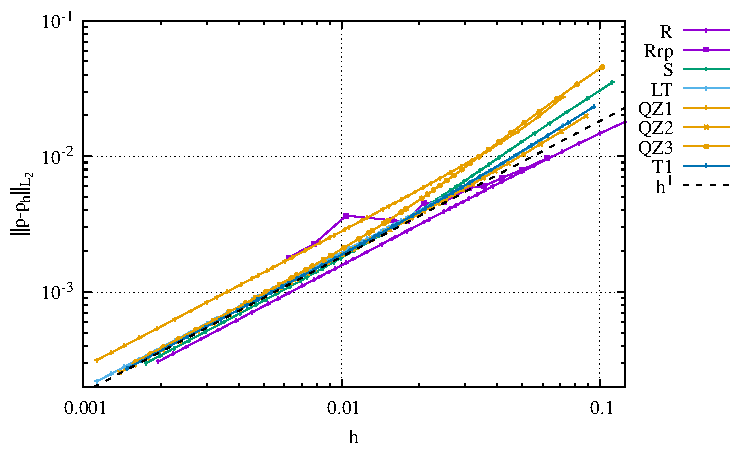
\includegraphics[width=8cm]{../results/errors_p_exp5}
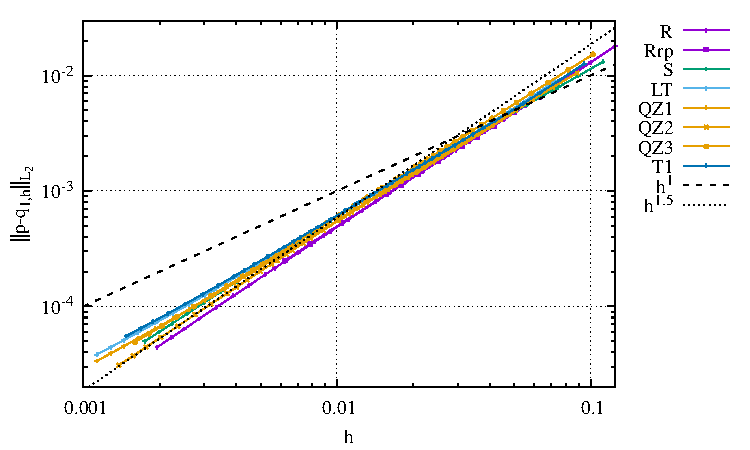
\includegraphics[width=8cm]{../results/errors_q1_exp5}
\caption{SolKz benchmark: velocity error, 
root mean square velocity, elemental pressure error and nodal pressure error
as a function of the the average mesh size $h$.} 
\label{fig:ressolkz}
\end{figure}










%%%%%%%%%%%%%%%%%%%%%%%%%%%%%%%%%%%%%%%%%%%%%%%%%%%%%%%%%%
\section{Buoyancy-driven flow}





%paragraph for non geo ppl
What often characterizes geodynamical modelling is the buoyancy-driven nature of the flow 
in the presence of a very strong hydrostatic pressure and a relatively small dynamic pressure.
On long periods of time the mantle and the lithosphere behave like non-Newtonian fluids
which effective viscosity ranges from about $10^{19}$ up to $10^{28}\si{\pascal\second}$, 
typical velocities are of the order of $1\si{\cm\per year}$, and pressure ranges from 
the atmospheric pressure at the surface ($\sim 10^5 \si{\pascal}$) up to about $100\si{\giga\pascal}$ 
at the core mantle boundary. The mantle is not well mixed and therefore not homeogenous: 
Subducted plate remnants which are colder than their surroundings are thought to slowly sink 
while thermo-chemical instabilities at the core mantle boundary are the location where 
so-called plumes root and traverse the mantle upwards.

The $Q_1\times P_0$ has been the workhorse of computational geodynamics for decades with 
very popular mantle convection and lithosphere deformation codes such as Citcom, SOPALE, 
UnderWorld, DOUAR \cite{brtf08}, FANTOM \cite{thie11}, ... FINISH



The following experiment is an idealised geodynamical setup.
The domain is a square of size $L_x=L_y=512$km filled with a fluid (the ``mantle'')
of density $\rho_1=3200\si{\kg\per\cubic\metre}$ 
and viscosity $\eta_1=10^{21}\si{\pascal\second}$.
A square block of size $128\times 128\si{\km}$ is placed in the domain and
is centered at location ($x_c,y_c$)=($256\si{\km}$, $384\si{\km}$) so 
as to insure that its sides
align with cell boundaries at all resolutions (we thereby wish to avoid
cases where the quadrature points inside an element would have different
density or viscosity associated to them). It is filled with a fluid
of density $\rho_2=\rho_1+\delta \rho$ and viscosity $\eta_2=10^{23}\si{\pascal\second}$.
The gravity vector points downwards with $|{\bm g}|=10\si{\metre\per\square\second}$. 
Boundary conditions are free slip on all sides.
This benchmark is similar or identical to the ones presented in 
\cite{mamo08}, \cite{gery10}, \cite{thie11} and \cite{sctc20}.

Density variations are often small compared to the density of the mantle itself
and they can be positive or negative: in a geodynamical context, 
the block could be interpreted as a detached slab
($\delta\rho>0$) or a plume head ($\delta\rho<0$). 
We here choose $\delta \rho=+8\si{\kg\per\cubic\metre}$, i.e. $\delta \rho/\rho_1 = 0.25\%$.

This experiment was run for resolutions $16m\times 16m$ with $m=\{1,2,3,4,5\}$. 
The vertical component of the velocity on a vertical line passing through the middle
of the domain is recorded and plotted in Fig.~\ref{fig:profiles}. 
There is no analytical solution to this problem so 
these values are plotted against a high resolution profile obtained with the state-of-the-art geodynamics ASPECT 
code\cite{krhb12,hedg17} based on the deal.II FE library \cite{XX} 
using a mesh of $128\times128$ $Q_2\times P_{-1}$ elements.


\begin{figure}[t]
\centering
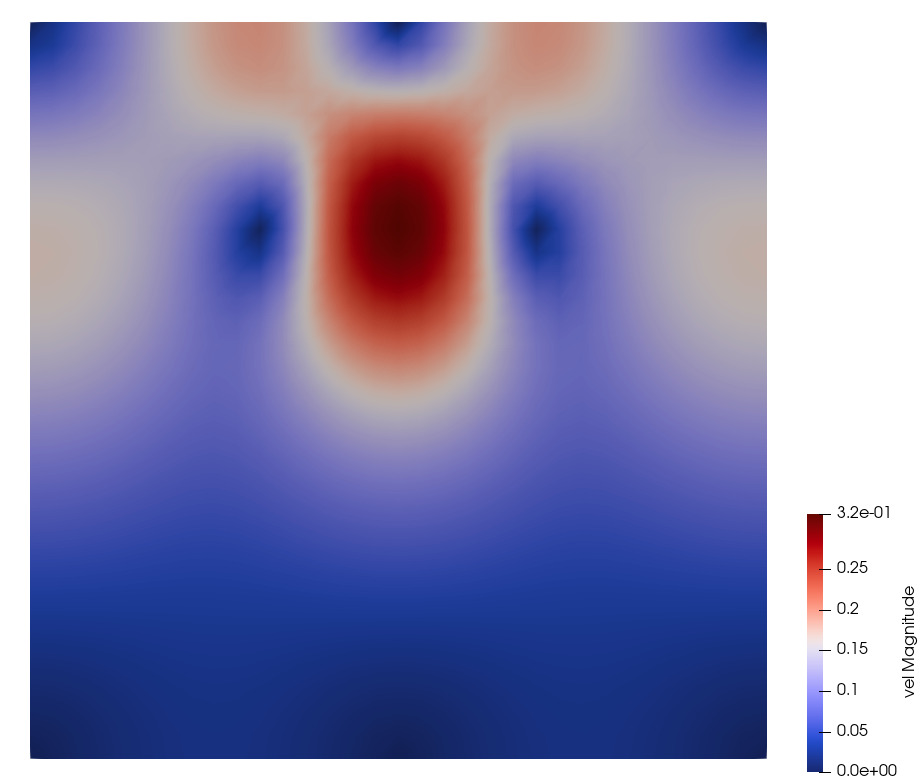
\includegraphics[width=4cm]{../results/sinking_block/figure_full/vel0.png}
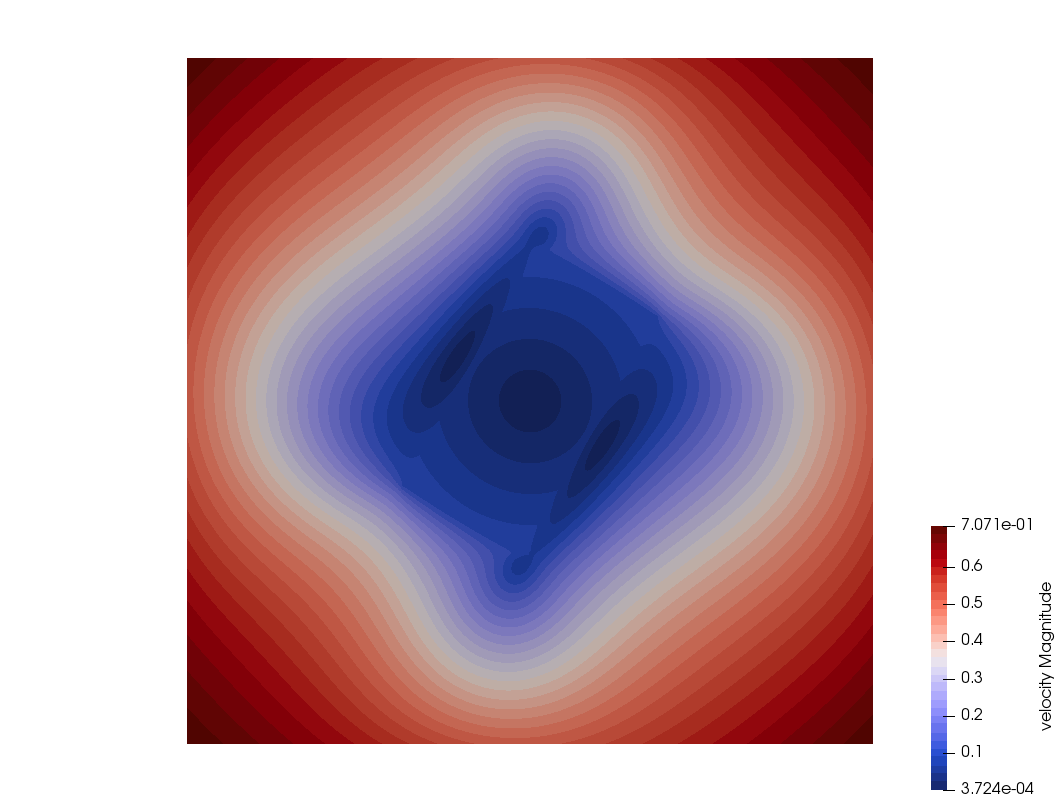
\includegraphics[width=4cm]{../results/sinking_block/figure_full/vel1.png}
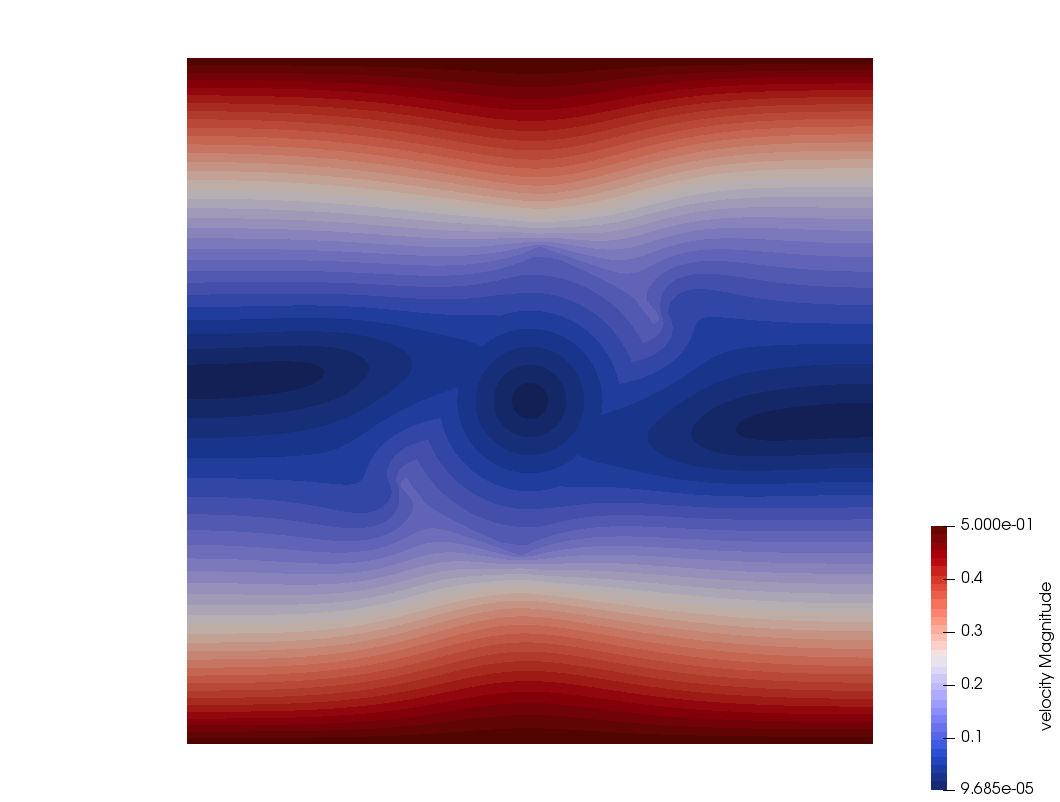
\includegraphics[width=4cm]{../results/sinking_block/figure_full/vel2.png}
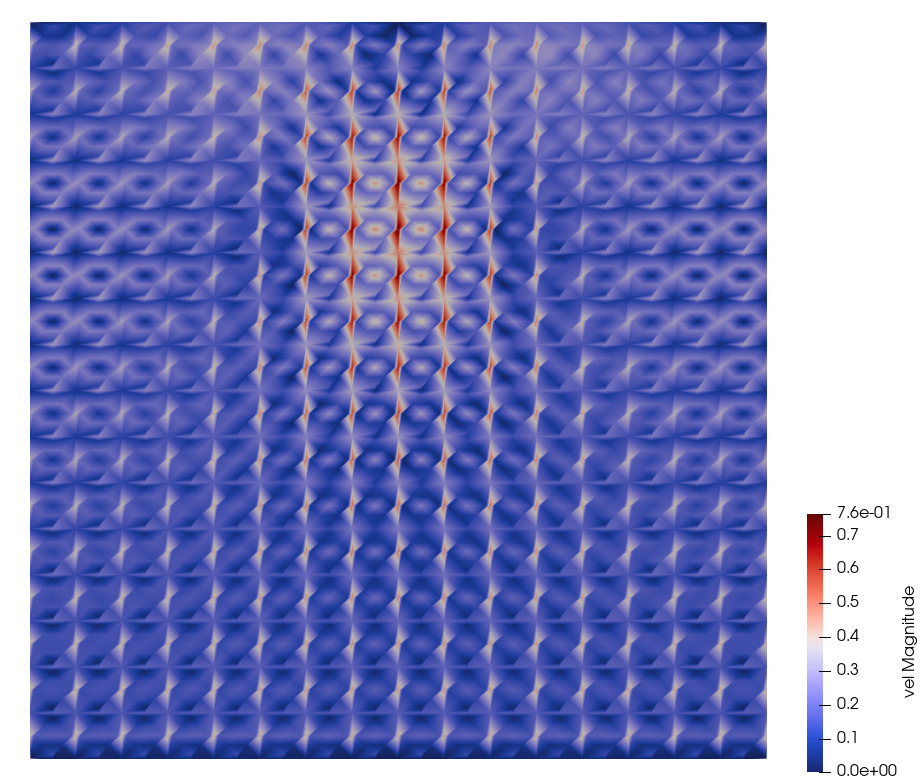
\includegraphics[width=4cm]{../results/sinking_block/figure_full/vel3.png}\\
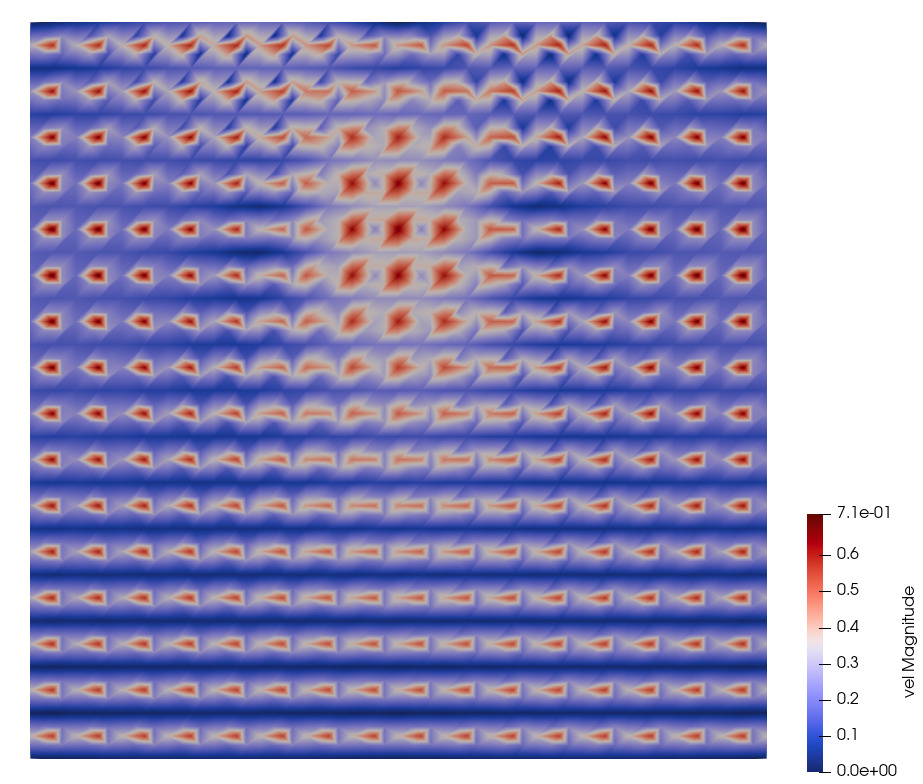
\includegraphics[width=4cm]{../results/sinking_block/figure_full/vel4.png}
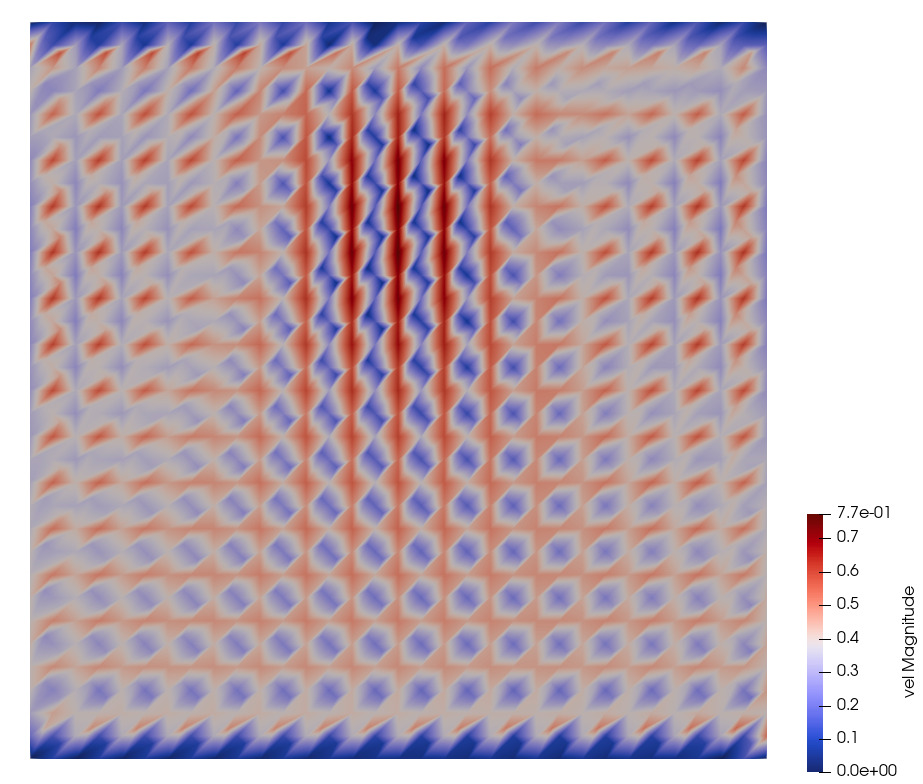
\includegraphics[width=4cm]{../results/sinking_block/figure_full/vel5.png}
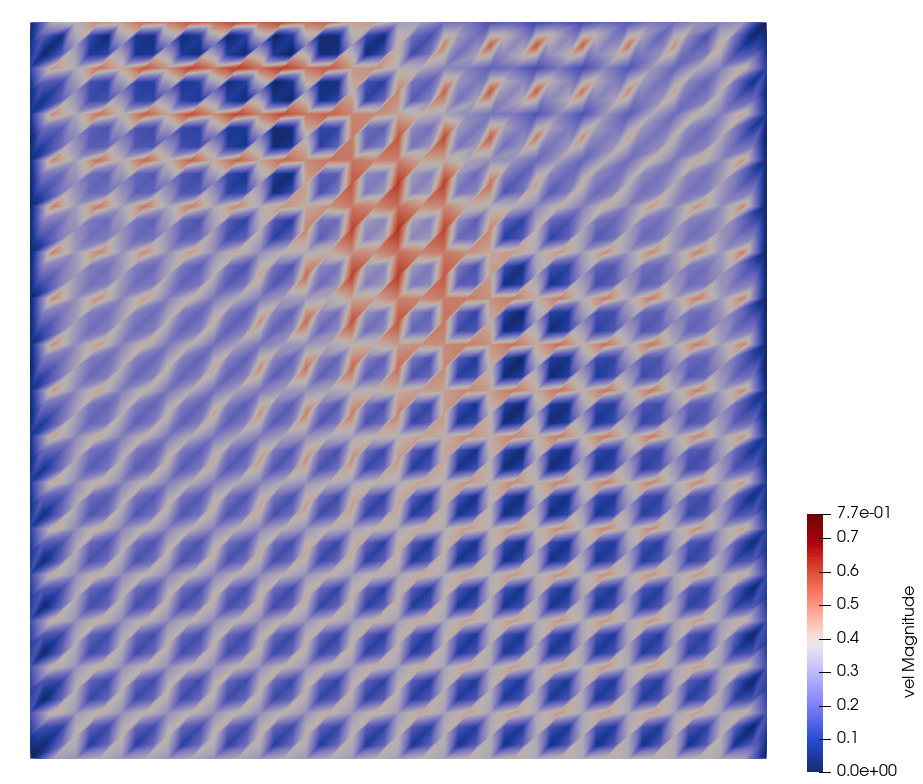
\includegraphics[width=4cm]{../results/sinking_block/figure_full/vel6.png}
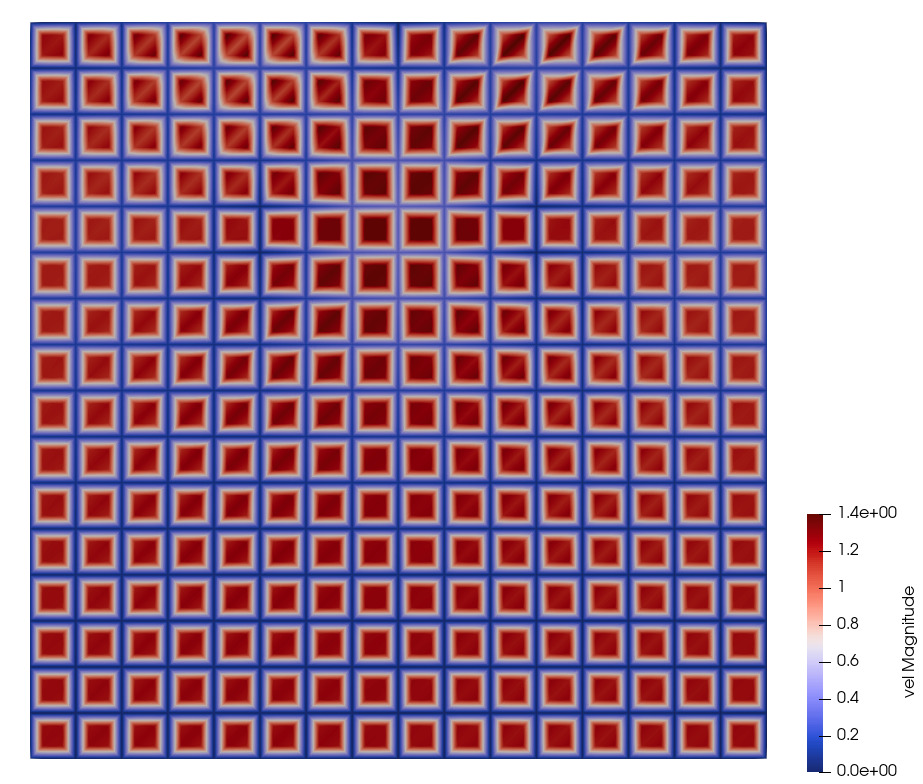
\includegraphics[width=4cm]{../results/sinking_block/figure_full/vel7.png}
\caption{Sinking block experiment with full densities: velocity fields 
obtained with meshes composed of $16\times 16$ macro-elements. \label{fig:dh1}}
\end{figure}


\begin{figure}[t]
\centering
\includegraphics[width=4cm]{../results/sinking_block/figure_reduced/vel.0000.png}
\includegraphics[width=4cm]{../results/sinking_block/figure_reduced/vel.0001.png}
\includegraphics[width=4cm]{../results/sinking_block/figure_reduced/vel.0002.png}
\includegraphics[width=4cm]{../results/sinking_block/figure_reduced/vel.0003.png}\\
\includegraphics[width=4cm]{../results/sinking_block/figure_reduced/vel.0004.png}
\includegraphics[width=4cm]{../results/sinking_block/figure_reduced/vel.0005.png}
\includegraphics[width=4cm]{../results/sinking_block/figure_reduced/vel.0006.png}
\includegraphics[width=4cm]{../results/sinking_block/figure_reduced/vel.0007.png}\\
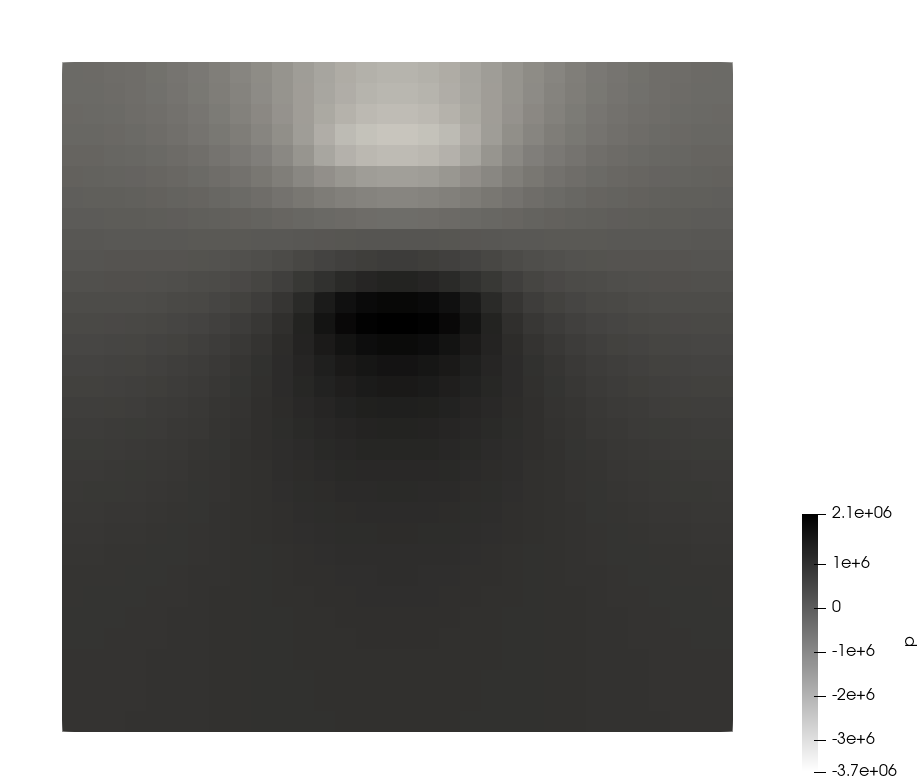
\includegraphics[width=4cm]{../results/sinking_block/figure_reduced/press.0000.png}
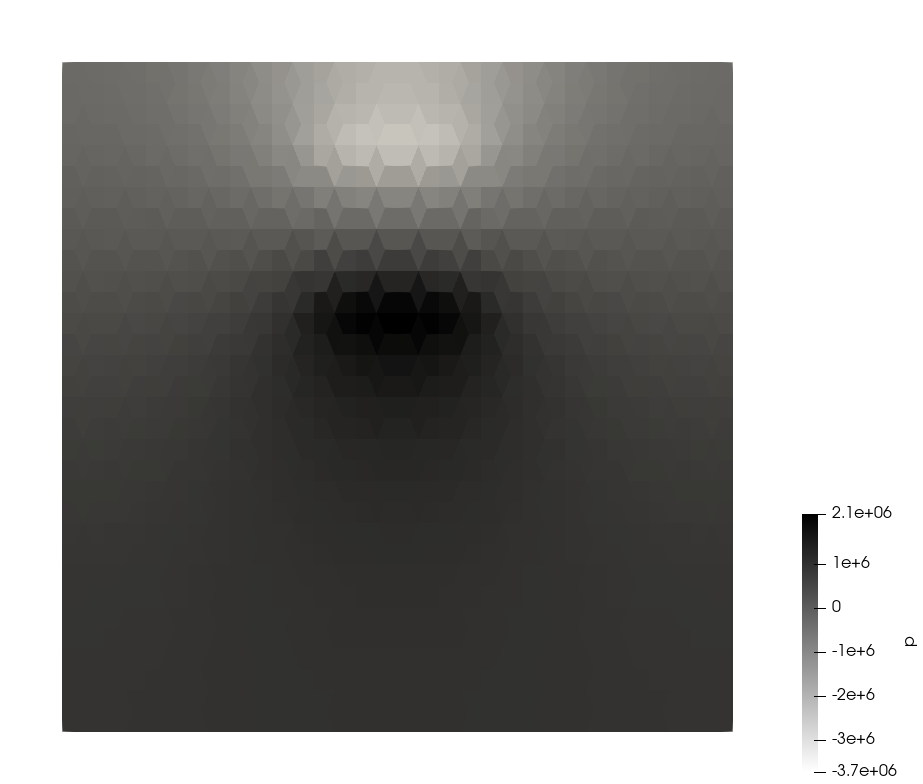
\includegraphics[width=4cm]{../results/sinking_block/figure_reduced/press.0001.png}
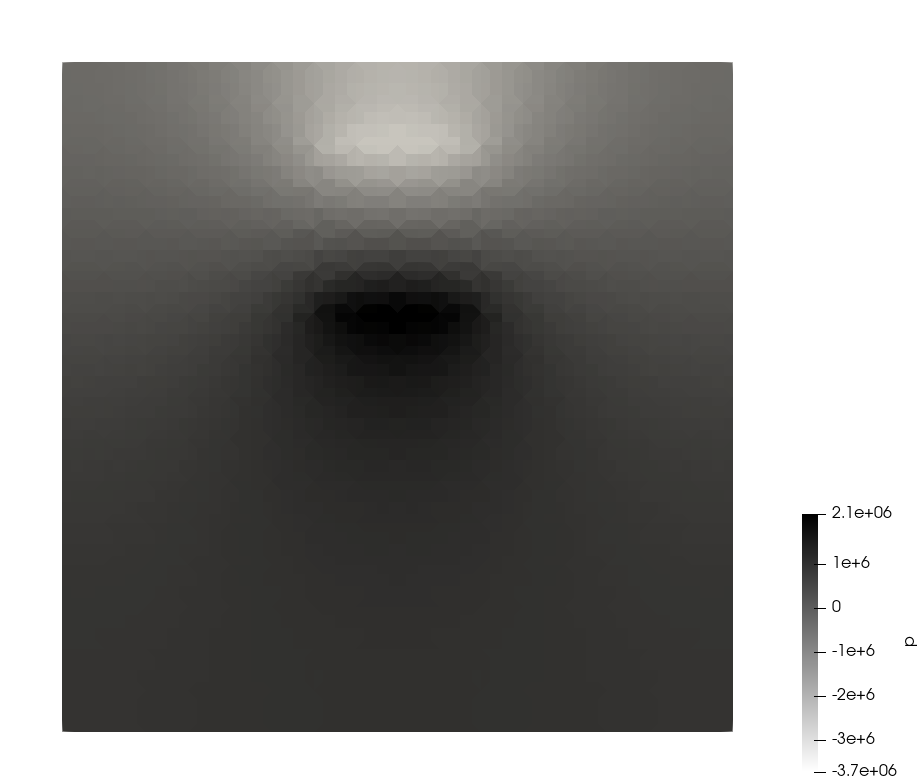
\includegraphics[width=4cm]{../results/sinking_block/figure_reduced/press.0002.png}
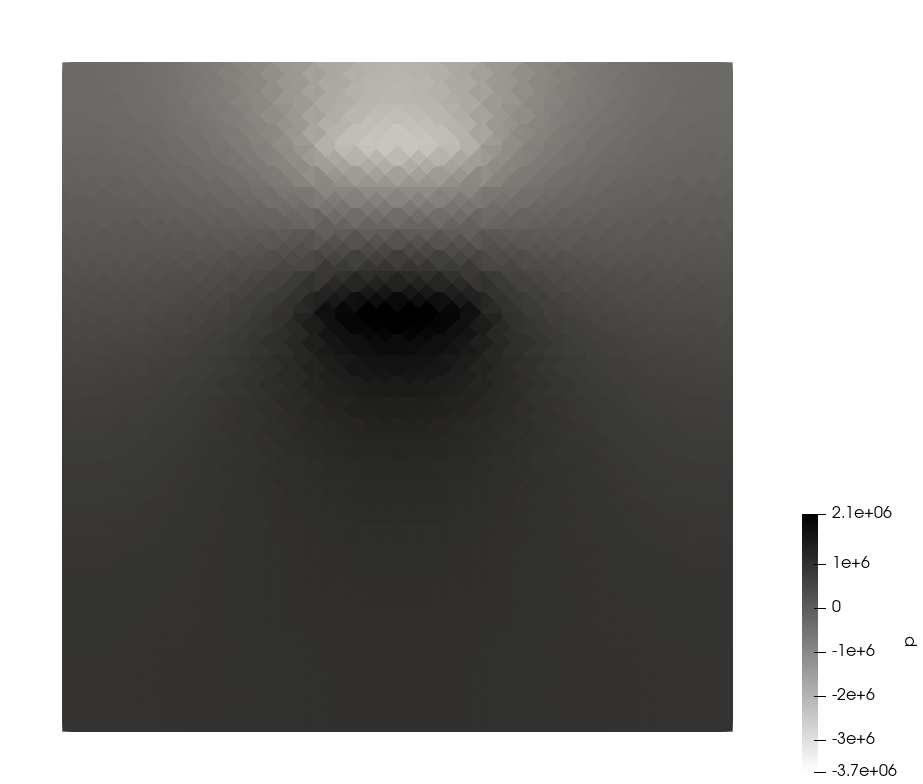
\includegraphics[width=4cm]{../results/sinking_block/figure_reduced/press.0003.png}\\
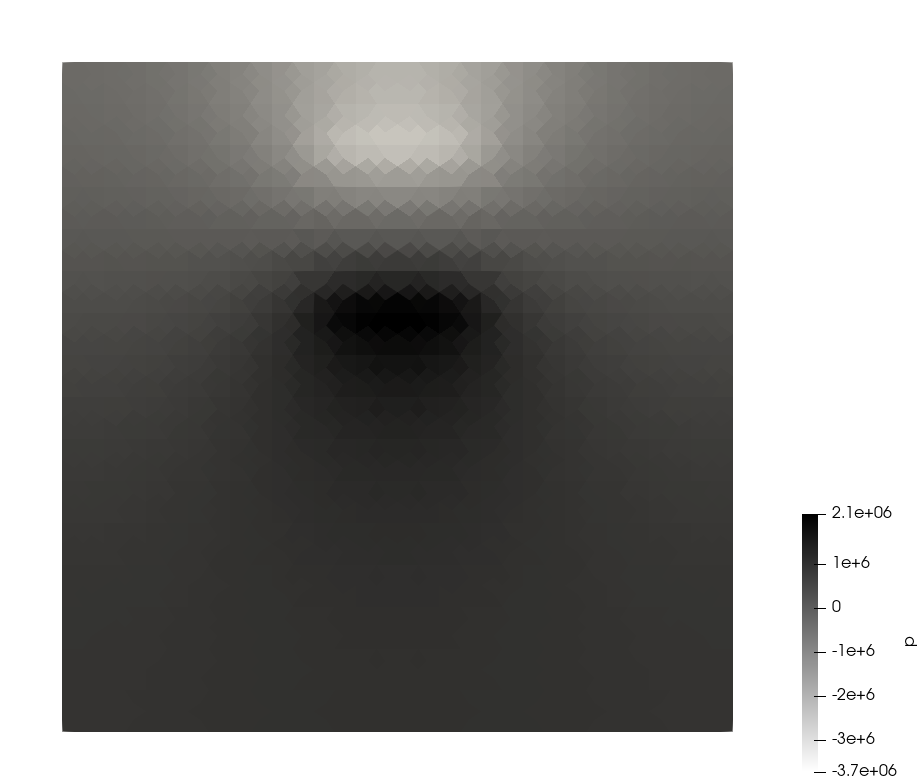
\includegraphics[width=4cm]{../results/sinking_block/figure_reduced/press.0004.png}
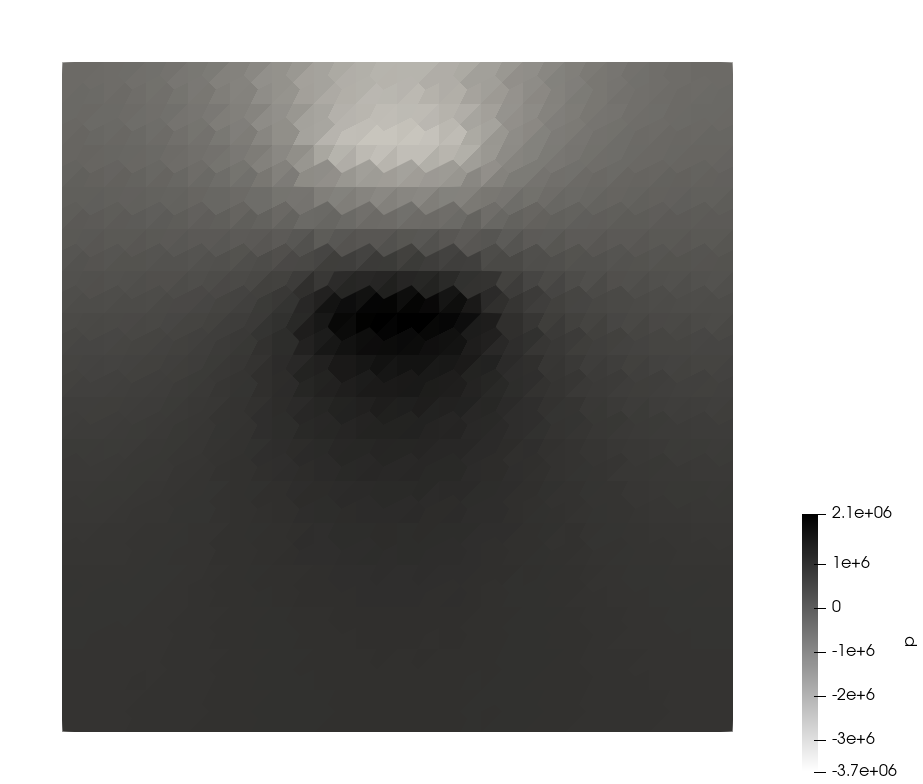
\includegraphics[width=4cm]{../results/sinking_block/figure_reduced/press.0005.png}
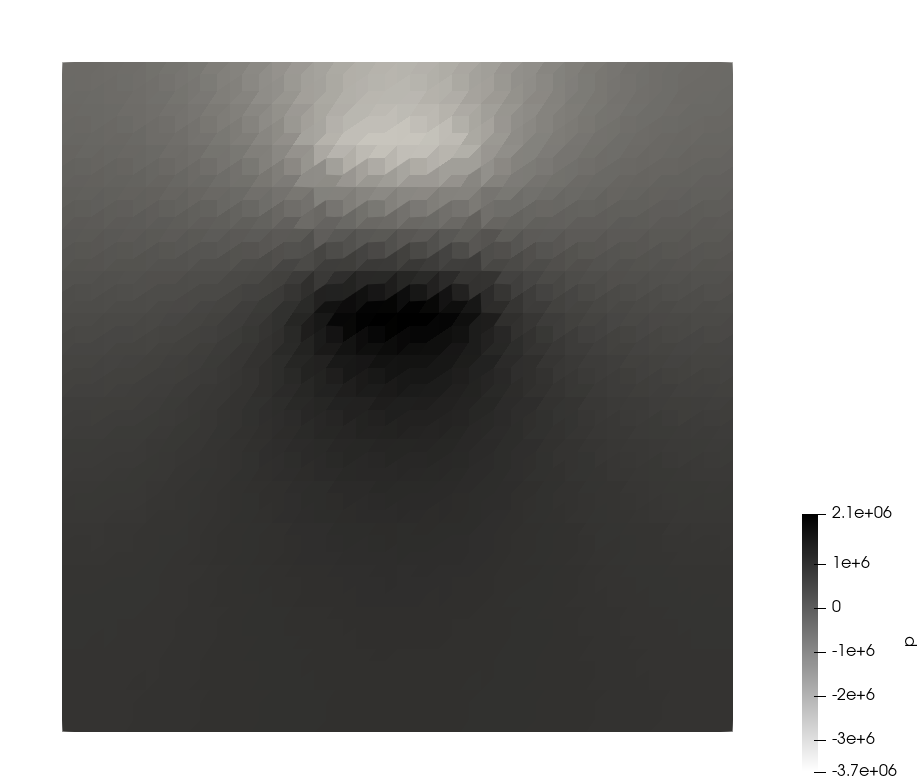
\includegraphics[width=4cm]{../results/sinking_block/figure_reduced/press.0006.png}
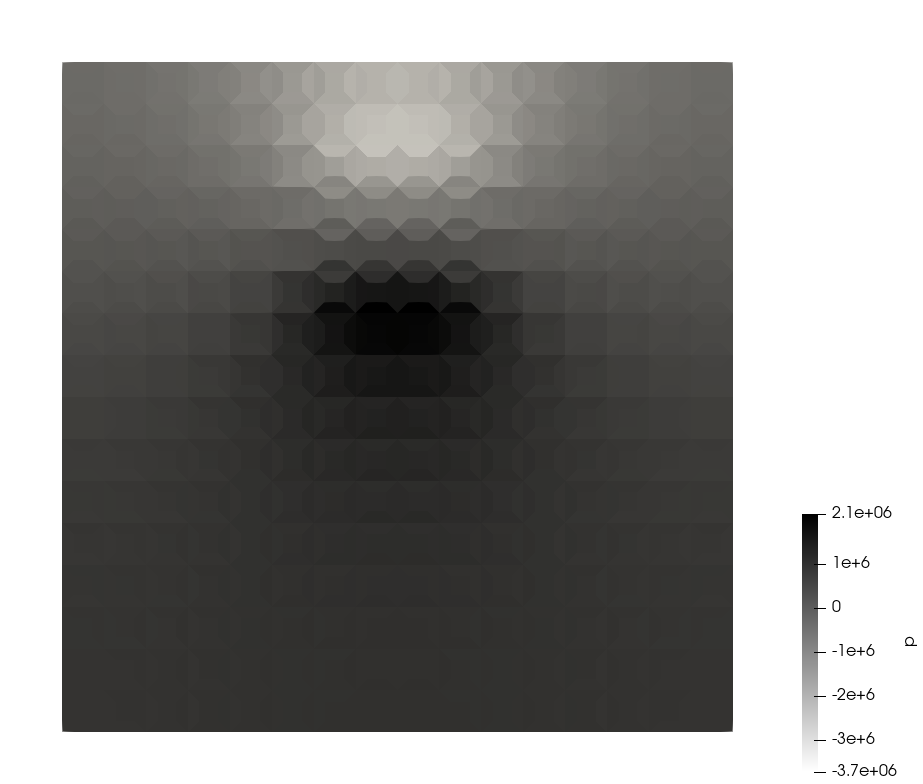
\includegraphics[width=4cm]{../results/sinking_block/figure_reduced/press.0007.png}\\
\caption{Sinking block experiment with reduced densities: velocity fields 
obtained with meshes composed of $16\times 16$ macro-elements. \label{fig:dh2}}
\end{figure}






\begin{figure}
\centering
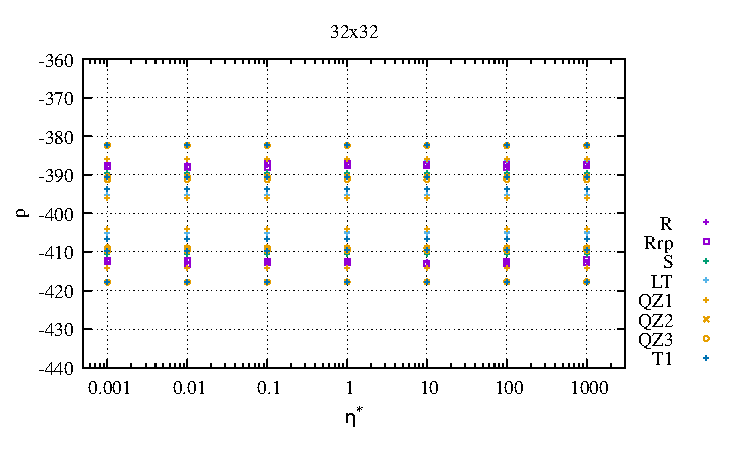
\includegraphics[width=8cm]{../results/sinking_block/p_block_res32.pdf}
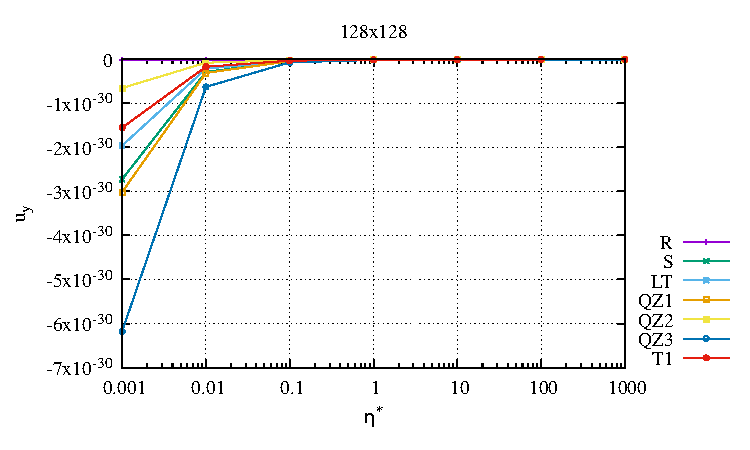
\includegraphics[width=8cm]{../results/sinking_block/v_block_res32.pdf}\\
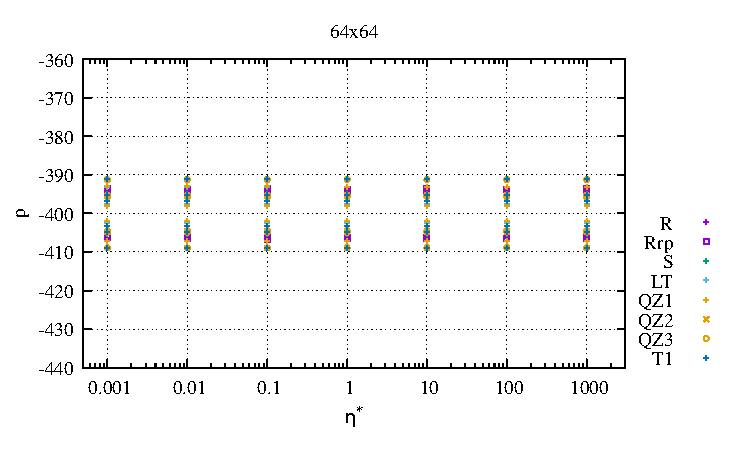
\includegraphics[width=8cm]{../results/sinking_block/p_block_res64.pdf}
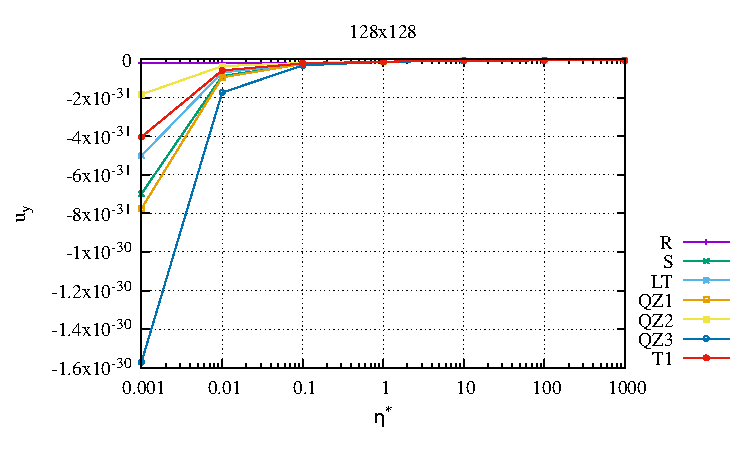
\includegraphics[width=8cm]{../results/sinking_block/v_block_res64.pdf}\\
\includegraphics[width=8cm]{../results/sinking_block/v_profile_res32.pdf}
\includegraphics[width=8cm]{../results/sinking_block/v_profile_res64.pdf}
\caption{Sinking block experiment with full density: } \label{fig:resblock}
\end{figure}







We find that
\begin{itemize}
\item no checkerboard ! 
\item All bad, except Reg and B!!!
\item results for QZ1,2,3, A, B not shown because quantitatively and qualitatively similar to those shown here.
\end{itemize}








%%%%%%%%%%%%%%%%%%%%%%%%%%%%%%%%%%%%%%%%%%%%%%%%%%%%%%%%%%%%%%%%%%%
\section{Conclusions}\label{sec5}

Conclusions about mms:

similar conclusions hold for other isoviscous mms. TEST




Conlcusions about buoyancy-driven flows:

macro-e have two advantages: no checkerboard modes AND stable. So CG applied to Schur should converge in a number of iterations independent of h. test with ELEFANT-2 ?

use in geodynamics possible IF reduced density or rather high resolution (but then why not Q2Q1). S is probably best overal.

awkward with particle-in-cell , inner structure of macro-element could influence shear band angle. 

also, if used at high res, full density, what about mesh deformation?

can we extend all/some to 3D? stability proof ?

q1 vs q2. in practice doe snot make much difference

if direct solver is used a sloan algo is needed

we do not consider penalty formulations (no choice of lambda)

Note that other q projections are available.

%compute indicator (eigenvalue, ... ?) for meshes and rank them ? see chappelle bathe

%I need to understand how to prove LBB stability and apply it to 3D elts ?

%I disregard randomised regular meshes bc how much random is not clear.


\printbibliography


\end{document}
